\chapter{Theoretische Grundlagen}
\label{chap:theorie}

%%%% Ein kleines Chapter zur schwachen WW??
%%%% Etwas zum solaren Neutrinoproblem??
%%%% SN1987A kurz mal erwähnen
%%%% Seesaw-Mechanismus erwähnen

\section{Geschichte der Neutrinos}
\label{sec:neutrinogeschichte}

Neutrinos wurden erstmals am $4.$ Dezember $1930$ von Pauli als Spin-$\frac{1}{2}$-Teilchen postuliert, um das Problem der Drehimpulserhaltung und das kontinuierliche Elektronenspektrum beim $\beta$-Zerfall zu lösen. %\cite{zuber}
Er führte das Neutrino als Teilchen ein, dass beim $\beta^-$-Zerfall
\begin{equation*}
    n \rightarrow p + e^- + \bar{\nu}_e
\end{equation*}
gemeinsam mit dem Elektron emittiert wird, anders als dieses allerdings nicht detektierbar ist. \\
Diese Annahme Paulis wurde lange kritisch betrachtet, bis Neutrinos in den $50$er Jahren in Atomreaktoren zweifellos nachgewiesen werden konnten. %\cite{zuber}\\

Im Standardmodell der Teilchen sind Neutrinos als einzige masselose, elektrisch neutrale Leptonen vertreten.
Theoretisch lassen sie sich durch die Wellenfunktionen $\psi$ als lorentzinvariante Lösung der relativistischen Diracgleichung
\begin{equation}
    \left(i \gamma_\mu \frac{\partial}{\partial x_\mu} - m \right) \psi = 0
    \label{eq:dirac}
\end{equation}
beschreiben.
Die Wellenfunktion ist dabei ein vierkomponentiger Spinor, $\gamma_\mu$ sind die $4 \times 4$-Gammamatrizen in Diracdarstellung mit
\begin{align}
    \gamma^0_\text{Dirac} = \left( \begin{array}{c c}
        \mathbb{1} & 0          \\ 
        0          & -\mathbb{1} \\ 
        \end{array}\right) \,,
    &&
    \gamma^k_\text{Dirac} = \left( \begin{array}{c c}
        0           & \sigma_k  \\ 
        -\sigma_k   & 0         \\ 
        \end{array}\right) \,,
    \label{eq:gammamatrizen}
\end{align}
wobei $\mathbb{1}$ die Einheitsmatrix und $\sigma_k$ mit $k = 1, 2, 3$ die $2 \times 2$-Paulimatrizen
\begin{align}
    \sigma_1 = \left( \begin{array}{c c}
        0 & 1   \\ 
        1 & 0   \\ 
        \end{array}\right) \,,
    &&
    \sigma_2 = \left( \begin{array}{c c}
        0           & -i  \\ 
        i  & 0         \\ 
        \end{array}\right) \,,
    &&
    \sigma_3 = \left( \begin{array}{c c}
        1           & 0 \\ 
        0   & -1         \\ 
        \end{array}\right)
    \label{eq:paulimatrizen}
\end{align}
darstellen. 

Somit sind Neutrinos auch die einzigen Leptonen, die nicht nur nicht stark wechselwirken, sondern auch nicht an der elektromagnetischen Wechselwirkung teilnehmen.
Tatsächlich ist ihre Wechselwirkung mit Materie so gering, dass die $7 \cdot 10^{10}$  Neutrinos, die pro $\si{\centi\meter}^2$ und pro Sekunde auf die Erde treffen, keinerlei Auswirkung
auf das Leben ihrer Bewohner haben \cite[S. ~133]{grupen}. 

Zu jeder der drei Leptonengenerationen, sprich Elektronen, Myonen und Tauonen existiert dabei ein korrespondierendes Neutrino.
Dieser sogenannte Flavour eines Neutrinos ist dabei nicht fest, sondern kann sich zeitlich und räumlich periodisch ändern.
Die Entdeckung dieser sogenannten Neutrinooszillationen erhielt im Jahre $2015$ den Nobelpreis \cite[S. ~19]{oberauer}.



\section{Neutrinos und spontane Symmetriebrechung}

Um die Masse der Neutrinos zu erklären, führen wir ein Quantenfeld ein, das Majoronenfeld, welches die Leptonenzahlsymmetrie, wenn auch nur geringfügig, bricht.
Dazu sollen hier zunächst einige Begrifflichkeiten geklärt werden.

\subsection{Das Eichprinzip} %\cite{kleingrot}

Das Prinzip der Eichinvarianz beschreibt Transformationen, die die Physik eines Systems, also die Lagrangedichte, invariant lassen.
Dabei unterscheiden wir zwischen globalen Transformationen, die sich, unabhängig von Raum und Zeit, überall gleichartig auf das System auswirken und lokalen Eichtransformationen, 
die von Ort und Zeit abhängig unterschiedlich auf das System wirken.

Für uns sind im Folgenden insbesondere die globalen Symmetrien relevant.
Jede dieser globalen Symmetrien, ist durch das Noether-Theorem mit einer Erhaltungsgröße verknüpft.
Unter globale Transformationen fallen beispielsweise die Multiplikation der Lösung $\psi$ der Schrödingergleichung um eine konstante komplexe Phase $\mathrm{e}^{i \alpha}$.

\subsection{Spontane Symmetriebrechung} %\cite{kleingrot}


Der Mechanismus der spontanen Symmetriebrechung erlaubt uns, massebehaftete Eichbosonen einzuführen, ohne die Eichinvarianz der Lagrangedichte durch explizite Massenterme zu verlieren.
Konkret sprechen wir von einer spontanen Symmetriebrechung, wenn die grundlegenden Gleichungen eines Systems über eine Symmetrie verfügen, der der Grundzustand nicht folgt.

Das Majoronenfeld, also auch die dazugehörigen Eichbosonen, die Majoronen, lässt sich durch ein Potential einführen, dessen Vakuumerwartungswert (VEV), also der Zustand niedrigster Energie $E_\text{min}$ verschieden von null ist. \\
Wir fordern also, dass unser System, beschrieben durch den Hamiltonian $H$, invariant unter einer Transformation $U$ bleibt, sprich der Kommutator $[H, U]$ verschwindet.
Es gilt also auch
\begin{equation*}
    H U \ket{0} = U H \ket{0} = E_\text{min} U  \ket{0} 
\end{equation*}
und damit
\begin{equation*}
    U \ket{0}_i = \ket{0}_j \,, \quad i \neq j \,,
\end{equation*}
sofern mehrere entartete Zustände $\ket{0}_i$ existieren. \\
Die Transformation $U$ lässt das Vakuum $\ket{0}$ also nicht notwendigerweise invariant.

Das einfachste Potential mit diesen Eigenschaften besitzt die Form
\begin{equation}
    V(x) = -\frac{1}{2} \mu^2 x^2 + \frac{1}{4} \lambda x^4 \,, \quad \mu,\lambda > 0 \,.
\end{equation}
Offensichtlich ist dieses, auch Mexico-Hut-Potential genannte, Potential radialsymmetrisch.
Es existiert also ein Kreis mit Radius
\begin{equation*}
    x_0 = \sqrt{\frac{\mu^2}{\lambda}} \,,
\end{equation*}
auf dem die Zustände minimaler Energie verteilt sind.
\autoref{fig:mexicohutpot} zeigt eine Darstellung des Potentials in zwei Dimensionen.

\begin{figure}[H]
    \centering
    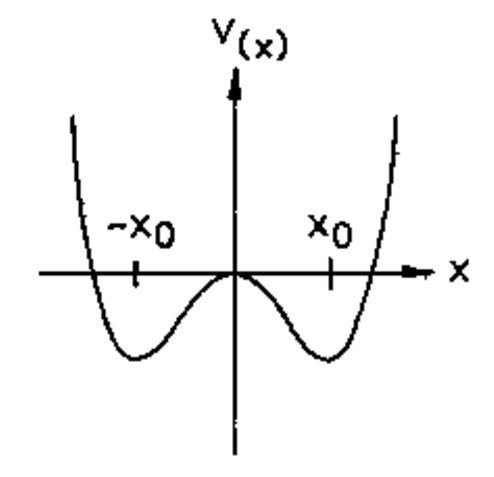
\includegraphics[]{figures/MexicoHutpotential.pdf}
    \caption{Darstellung des Mexico-Hut-Potentials in zwei Dimensionen. Zu erkennen sind die zwei möglichen Grundzustände $x = \pm x_0$ \cite{kleingrot}.}
    \label{fig:mexicohutpot}
\end{figure}

Anschaulich stellen wir uns vor, dass wir uns zunächst im Zentrum des Potentials befinden.
Von diesem Punkt aus besitzt das Potential eine globale Symmetrie, egal in welche Richtung wir schauen.
Betrachten wir das ganze aber von einem der Vakua, existiert diese Symmetrie unter der Transformation $x \rightarrow -x$ nicht länger.

\section{Ursprung der Neutrinomasse} %\cite{kleingrot}
\label{sec:neutrinomasse}

Als nur schwach wechselwirkende Teilchen ist zum jetzigen Zeitpunkt nur die Existenz linkshändiger Neutrinos $\nu_L$ und rechtshändiger Antineutrinos $\bar{\nu}_R$ bewiesen.
Diese sind über die Ladungs- und Paritätskonjugation $C P$ durch 
\begin{equation}
    (\nu_L)^{C P} = \bar{\nu}_R
    \label{eq:cpkonju}
\end{equation}
miteinander verknüpft.
Der Paritätsoperator $P$ transformiert dabei linkshändige in rechtshändige Teilchen und umgekehrt, die Ladungskonjugation überführt Teilchen in ihre Antiteilchen, ohne dabei ihre Händigkeit zu verändern.
Sind die ladungskonjugierten Teilchen zu $\nu_L$ bzw. $\bar{\nu}_R$ bisher nicht beobachtete, unabhängige Teilchen, sprechen wir von einem Dirac-Neutrino.
Ist $\nu_L$ bzw- $\bar{\nu}_R$ sein eigenes ladungskonjugiertes Teilchen, gilt also
\begin{align*}
    (\nu_L)^C = \nu_L \,, && (\bar{\nu}_R)^C = \bar{\nu}_R \,.
\end{align*}
Diese, nach dem italienischen Physiker Ettore Majorana benannten Majorana-Neutrinos lösen nach wie vor die Diracgleichung \eqref{eq:dirac}, es existieren allerdings nur zwei physikalisch unterscheidbare Zustände.
Diese beiden Majorana-Masseneigenzustände
\begin{align*}
    \nu_1 = \nu_L + \nu^{C P}_R \\
    \nu_2 = \nu_R + \nu^{C P}_L
\end{align*}
sind ihre eigenen Antiteilchen und bilden gemeinsam den Massenterm der Lagrangedichte $\mathcal{L}_M$ zu
\begin{equation}
    \mathcal{L}_M = \mathcal{L}^L_M + \mathcal{L}^R_M = -\frac{1}{2} m^M_L \bar{\nu}_1 \nu_1 - \frac{1}{2} m^M_R \bar{\nu}_2 \nu_2 \,.
    \label{eq:lagrangedichtemajo}
\end{equation}
Dabei stellen $m^M_L$ bzw. $m^M_R$ als Massen die Kopplungsstärken zwischen $\nu_L$ und $\bar{\nu}_R$ bzw. $\nu_R$ und $\bar{\nu}_L$ dar.

Im Standardmodell ordnet der Leptonenzahloperator $L$ jedem Lepton die Leptonenzahl $+1$ und jedem Antilepton die Leptonenzahl $-1$.
So erhalten auch Neutrinos im Standardmodell eine Leptonenzahl. 
Sind jetzt jedoch, wie oben beschrieben, Neutrinos und Antineutrino als Majoranateilchen identisch, ergibt die Zuordnung einer Leptonenzahl keinen Sinn mehr.
Die globale Leptonenzahlsymmetrie ist also, wenn auch nur sehr geringfügig, spontan gebrochen.











